% ================================================
% setting
% ================================================

% upLaTeXの環境でコンパイルの場合は"u"がつく
\documentclass[uplatex, 12pt, a4j]{ujreport}
% \documentclass[uplatex, 12pt, a4j, fleqn]{ujbook}

% begin.texに使用するパッケージなどの記述

% 読み込ませたいパッケージを記述する

% 太字が使える
\usepackage{bm}
%\usepackage{AIthesis}
% 図の関係で必要
\usepackage[dvipdfmx]{graphicx}

% pdf読み込みできるやつ
%\usepackage{mediabb}

% 数式のやつ
\usepackage{amsmath,amssymb}
\usepackage{amsthm}
\usepackage{longtable}
\usepackage{enumerate}
\usepackage{float}
\usepackage{wrapfig}
\usepackage{ascmac}
% 表に斜線を引ける、styファイルは要ダウンロード
%http://www.biwako.shiga-u.ac.jp/sensei/kumazawa/tex/slashbox.html
%\usepackage{slashbox}
% URLを直接記述できる、\url{}
\usepackage{url}
\usepackage{multirow}
\usepackage{ccaption}
\usepackage{afterpage}
\usepackage[a4paper]{geometry}
% 参考文献を本文で引用するときに使うやつ
\usepackage{cite}
% 図を横にならべて(a) OOとかできるやつ
\usepackage{subcaption}
% \usepackage[subrefformat=parens]{subcaption}
% まとめてコメントアウトできるやつ
\usepackage{comment}
% 表のセル内で自動改行するために必要
\usepackage{tabularx}
% 図の配置で[h]を指定した時に、確実にその位置に配置するやつ
\usepackage{here}
% \newpageで改ページ(文章変だけど)
\usepackage{afterpage}

% 図の配置を変えるやつ
%\usepackage[colorlinks=false,urlcolor=blue]{hyperref}




% 行数設定など行う
\makeatletter
\def\mojiparline#1{
    \newcounter{mpl}
    \setcounter{mpl}{#1}
    \@tempdima=\linewidth
    \advance\@tempdima by-\value{mpl}zw
    \addtocounter{mpl}{-1}
    \divide\@tempdima by \value{mpl}
    \advance\kanjiskip by\@tempdima
    \advance\parindent by\@tempdima
}
\makeatother
\def\linesparpage#1{
    \baselineskip=\textheight
    \divide\baselineskip by #1
}

% 余白の設定
% A4(297mm)
\setlength{\textheight}{227truemm}
\setlength{\headheight}{20truemm}
\setlength{\topskip}{20truemm}
\setlength{\headsep}{15truemm}
\setlength{\footskip}{10truemm}
\addtolength{\topmargin}{-1truein}

% セクションの番号付けの深さを設定
% 例えば3を指定すると、\subsubsubsectionまでは番号がつく
\setcounter{secnumdepth}{5}

% 図の保存場所
\graphicspath{{../fig/}}

% ================================================
% Document (start)
% ================================================

% ドキュメントの開始
\begin{document}

% 一行あたり文字数の指定
\mojiparline{35}
% 1ページあたり行数の指定
\linesparpage{27}


% タイトルの出力
% title.texを読み込んでる書いておく

% 表紙

\begin{titlepage}
	\begin{center}
		\vspace*{30truept}
		{\Large 令和5年度 卒業論文} \\
		\vspace{100truept}
		{\LARGE BinaryConnectを用いた}\\
		\vspace{12truept}
		{\LARGE コーヒー生豆の良否判定} 
		\vspace{80truept}\\
		{\large
		米子工業高等専門学校\\
		電子制御工学科 内田研究室\\
		}
		\vspace{50truept}
		{\large 学籍番号 19326}\\ % 学籍番号
	
		\vspace{10truept}
		{\large  橋本 恭輔}\\ % 著者
	
		\vspace{50truept}
		{\large 令和6年1月25日 提出}\\ % 提出日
	\end{center}
\end{titlepage}




% 図番号の後を":"をスペースに置き換える
% お好みで設定
\captionsetup{labelsep=space}
\renewcommand{\include}[1]{}
\renewcommand\documentclass[2][]{}

% 目次用にページ番号の付け方を"roman"に変えておく
\pagenumbering{roman}
% 目次の出力
\tableofcontents
% 図目次の表示
\listoffigures
% 表目次の表示
\listoftables

% 各チャプター分けしたファイルを読み込む

% ====================================
% chapter 1
% ====================================

\chapter{序章}

% ページ番号をリセット
\setcounter{page}{1}
% ページ番号の付け方をromanからarabicに変えておく
\pagenumbering{arabic}


\section{背景}

\subsection{コーヒーの需要}
コーヒーは世界中で様々な形で飲まれており,近年日本でもコーヒーの需要は増加傾向にある.図\ref{fig_syouhi}は日本国内における年間のコーヒー消費量の推移である.1996年以降コーヒー消費量は増加を続け2016年には47万[t]を超える消費量を見せている.特に嗜好品としてのコーヒーがブームを迎えており,スペシャルティコーヒーと呼ばれる品質を重視したコーヒーの需要が高まっている

スペシャルティコーヒーとは「消費者(コーヒーを飲む人)の手に持つカップの中のコーヒーの液体の風味が素晴らしい美味しさであり,消費者が美味しいと評価して満足するコーヒーであること.」と定義づけられており,カップの中の風味が素晴らしい美味しさであるためには,コーヒーの豆(種子)からカップまでの総ての段階において一貫した体制・工程・品質管理が徹底していることが必須であるとされている.具体的には生産国における管理・処理が適切になされ,適切な輸送と保管により劣化のない状態で焙煎された高品質なコーヒー豆を用いて適切な抽出が行われたものである必要がある.
\begin{figure}[]
  \begin{center}
    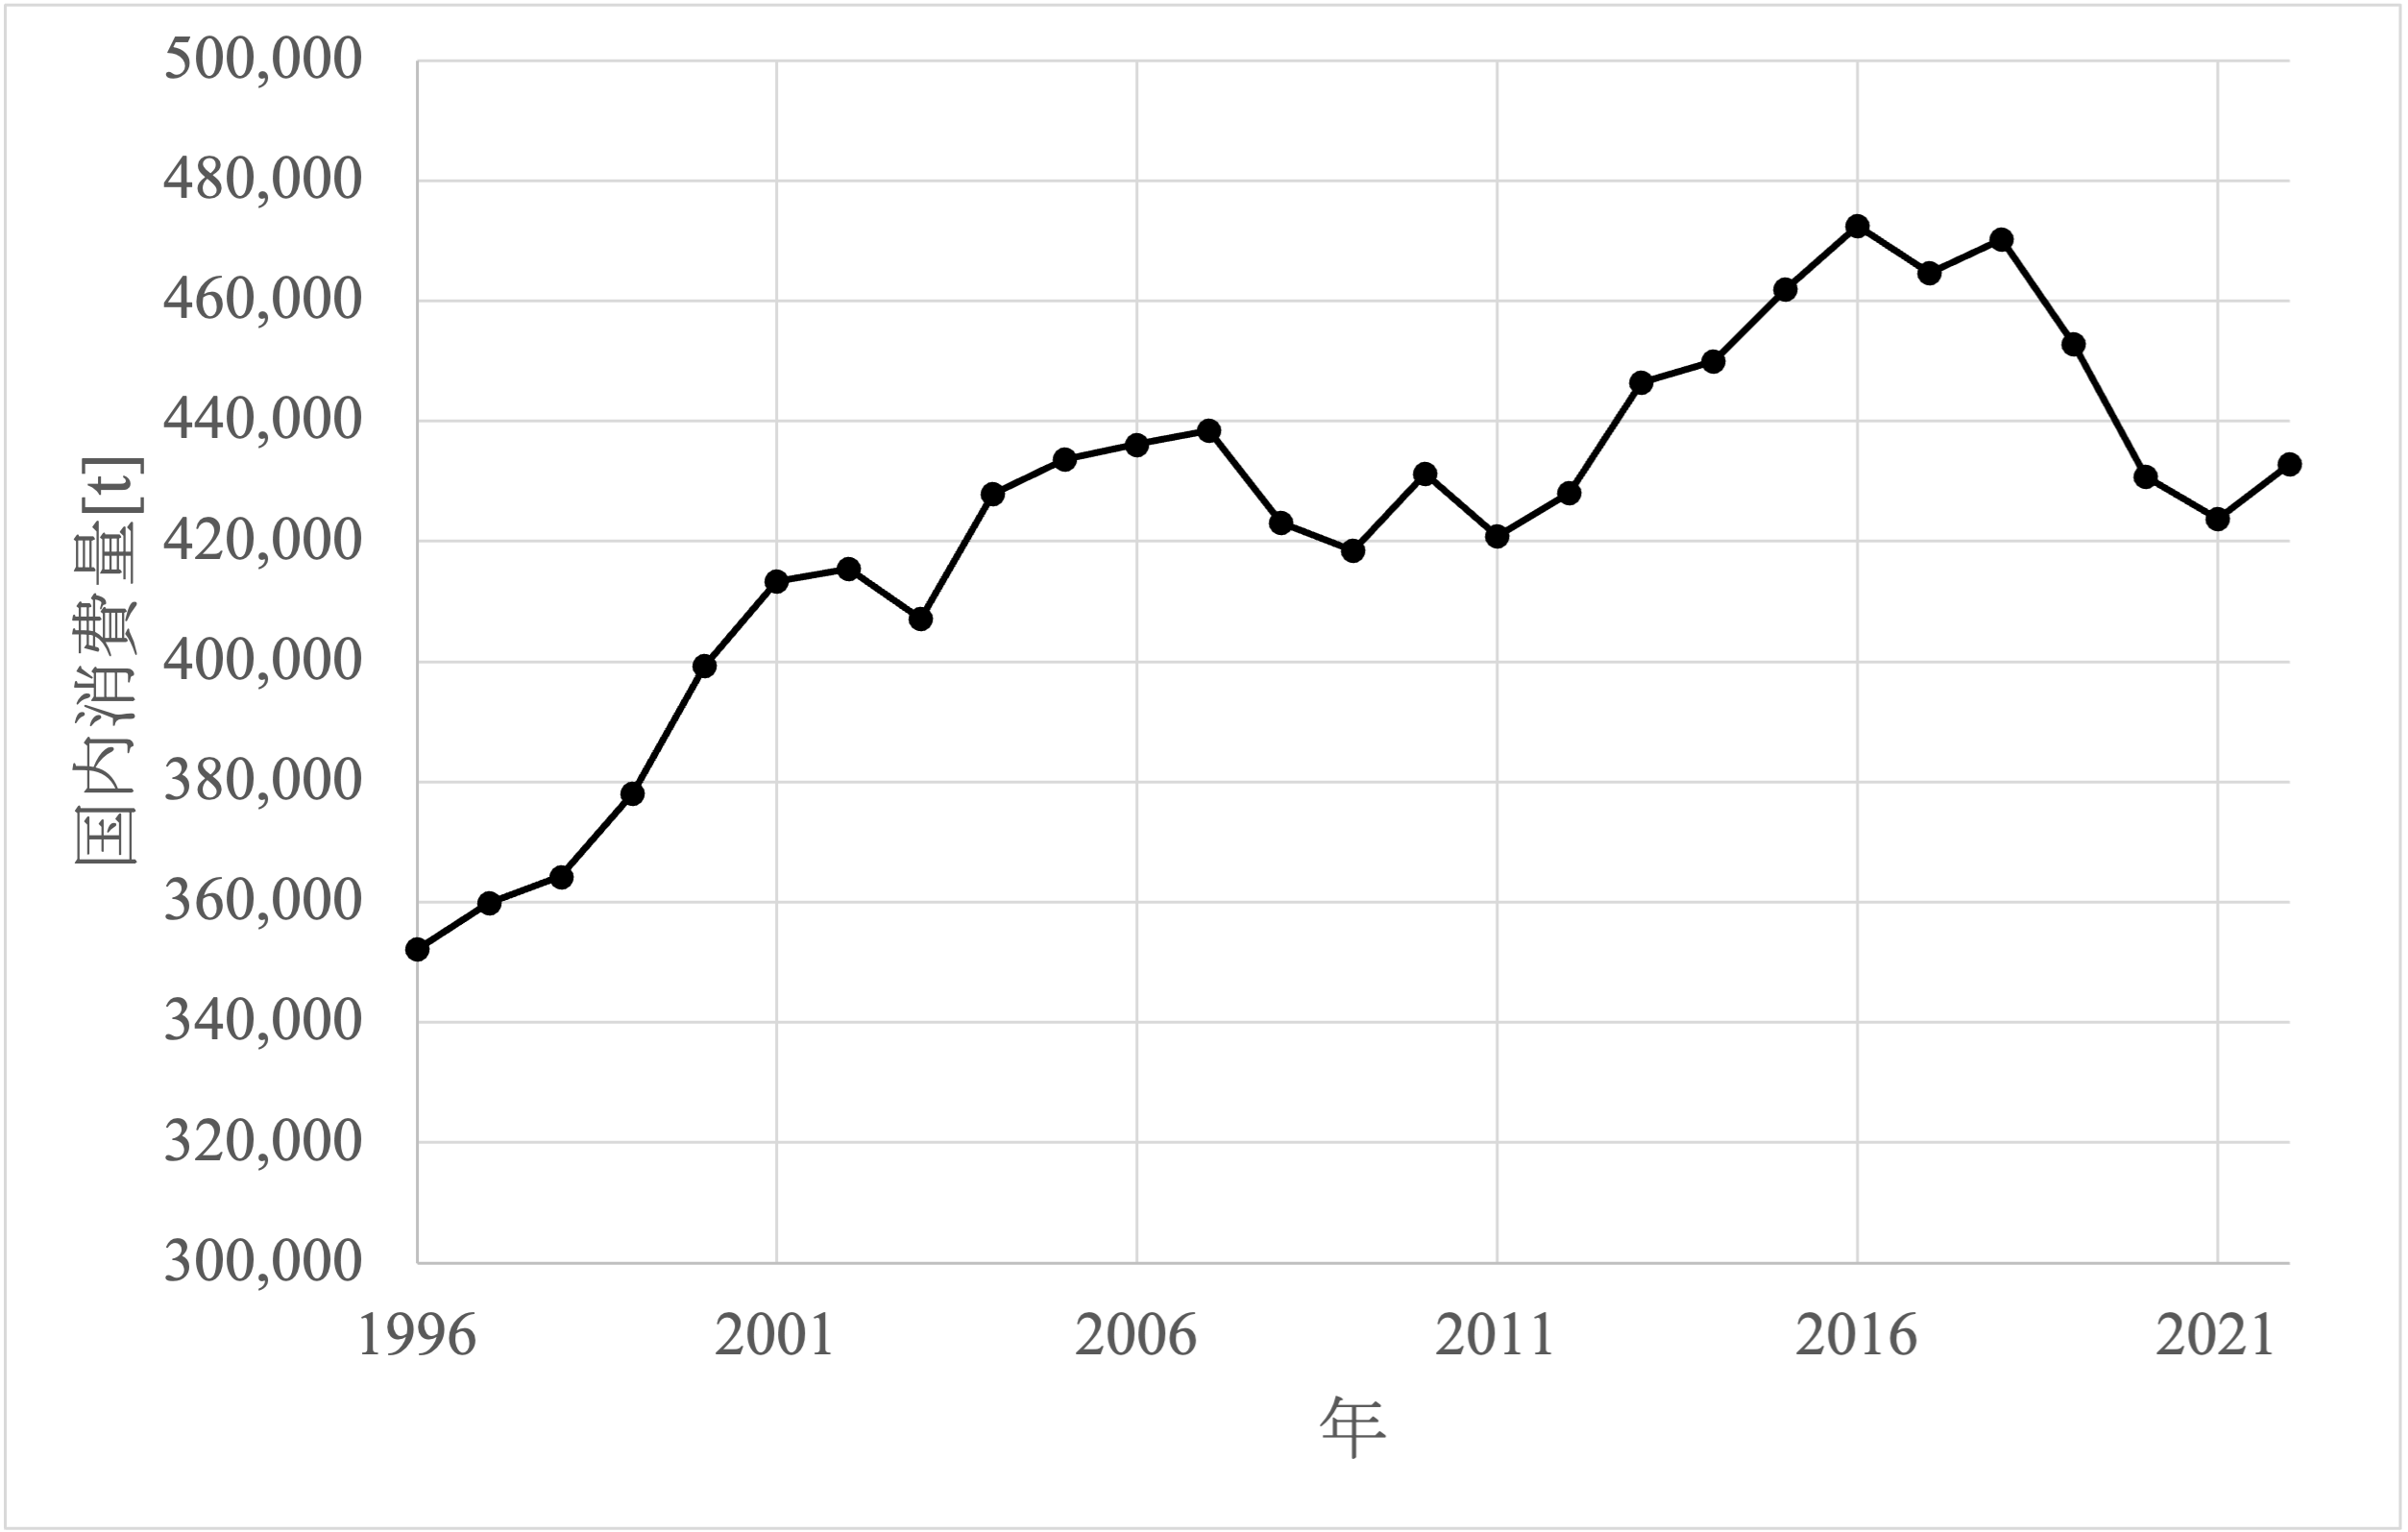
\includegraphics[scale = 0.5]{./chapter1/coffee_syouhi.png}
    \caption{Coffee consumption in Japan}
    \label{fig_syouhi}
  \end{center}
\end{figure}

\subsection{欠点豆とハンドピック}
近年のスペシャルティコーヒーのブームにより高品質なコーヒー豆が求められているが,コーヒー生豆において欠点豆と呼ばれるものが存在する.
欠点豆とはコーヒー生豆における,虫食いや欠けのあるような不良な豆のことである.以下に欠点豆の種類とその問題点についてまとめる.
\begin{itemize}
  \item カビ臭豆:不完全な乾燥や湿気を帯びた状態での輸送・保管が原因となり,青カビや白カビが発生した豆のこと.除去しなければコーヒー液自体にカビ臭が付着してしまう.
  \item 発酵豆:生産時や輸送中に発行が進み,菌が繁殖してしまっている豆のこと.異臭の原因になる.
  \item 貝殻豆:乾燥不良や異常勾配で発生する,センターカットから割れてしまった豆を指す.煎りムラの原因になり,焙煎時間が長くなると着火の危険性まで出てくる.
  \item 虫食い豆:コーヒーチェリーに産み付けられた蛾の幼虫がコーヒー豆の内部を食べることによってできた穴の空いたコーヒー豆のこと.濁りや異臭の原因になる.
  \item ピーベリー:発育不良によって通常コーヒーチェリー内部に2つあるコーヒー豆が1つの状態で育ってしまったもの.単体での味への影響はないが煎りムラの原因になる.
\end{itemize}
これらの欠点豆を選別しないまま焙煎を行なってしまうと煎りムラの原因や風味を劣化させる原因となってしまうため取り除く必要があるが,その際人間がコーヒー豆を目視で判別し手で取り除く「ハンドピック」と呼ばれるものを行なっている.
しかし,ハンドピックにはいくつかの問題が存在する.1つ目は生産地でハンドピックをすると,売り出すコーヒー豆の減少や作業量の増加からコーヒー豆の価格が高騰してしまうこと.2つ目は生産地でハンドピックをしたとしても輸送や保管の段階でコーヒー豆が劣化してしまい,輸入後のハンドピックが避けられないこと.3つ目はハンドピックそのものの労力が大きいことである.生産地から販売店までの商通で安価に精度良く選別することはできないため,販売店や個人でのハンドピックが必須であるが,それには大きな時間と労力が費やされている.

\section{目的}
ハンドピックにかかる大きな労力を低減するため,本研究では機械学習を用いてコーヒー生豆の良否判定を行う.先行研究ではConvolutional Neural Network(以下,CNN)を用いた判別を実現している.しかし,CNNの重みは浮動小数のため計算コストが高い.販売店や個人での利用を考えると,装置の小型化や省電力化が求められるため,将来的にFPGAやマイコンなどの計算リソースの少ないデバイスで制御したい.そこでBinaryConnectという手法を用いてNeural Network中の重みの2値化を目指す.通常,浮動小数で表されるCNNの重みは32bitや64bit分のメモリを消費するが,BinaryConnectを用いれば重みは1bitで表すことができる.これにより,メモリの消費を減らすことができるうえ,乗算機の数も減らすことができる.本稿ではCNNとBinalyConnectを用いてコーヒー生豆の良否判定精度を実験により比較し,BinaryConnectの有効性を検証する.


% ====================================
% chapter 2
% ====================================
\chapter{BinaryConnectによる良否判定}

% ******************************************************
% NeuralNetwork
% ******************************************************
\section{Neural Network}
Neural Networkとはニューロンと呼ばれる人間の脳細胞をもとに作られた数理モデルである.入力に対し重みをかけた時の出力から入力の特徴を抽出し分類問題を解く機械学習の1種である.


\subsection{Neural Networkの構造}
Neural Networkはユニットと呼ばれる最小要素を持ち,それに対し複数の入力と重み,バイアスから計算結果を出力する.
これらは図\ref{fig_NN1}のような構造をしており,入力$x_i$に対し重み$w_i$を乗算したものにバイアス$b$を足すことで出力$y$を得る.計算式は以下のように表される.
\begin{align}
y &= w_{1}x_{1} + w_{2}x_{2} + w_{3}x_{3} + b
\end{align}
\begin{figure}[htbp]
  \begin{center}
    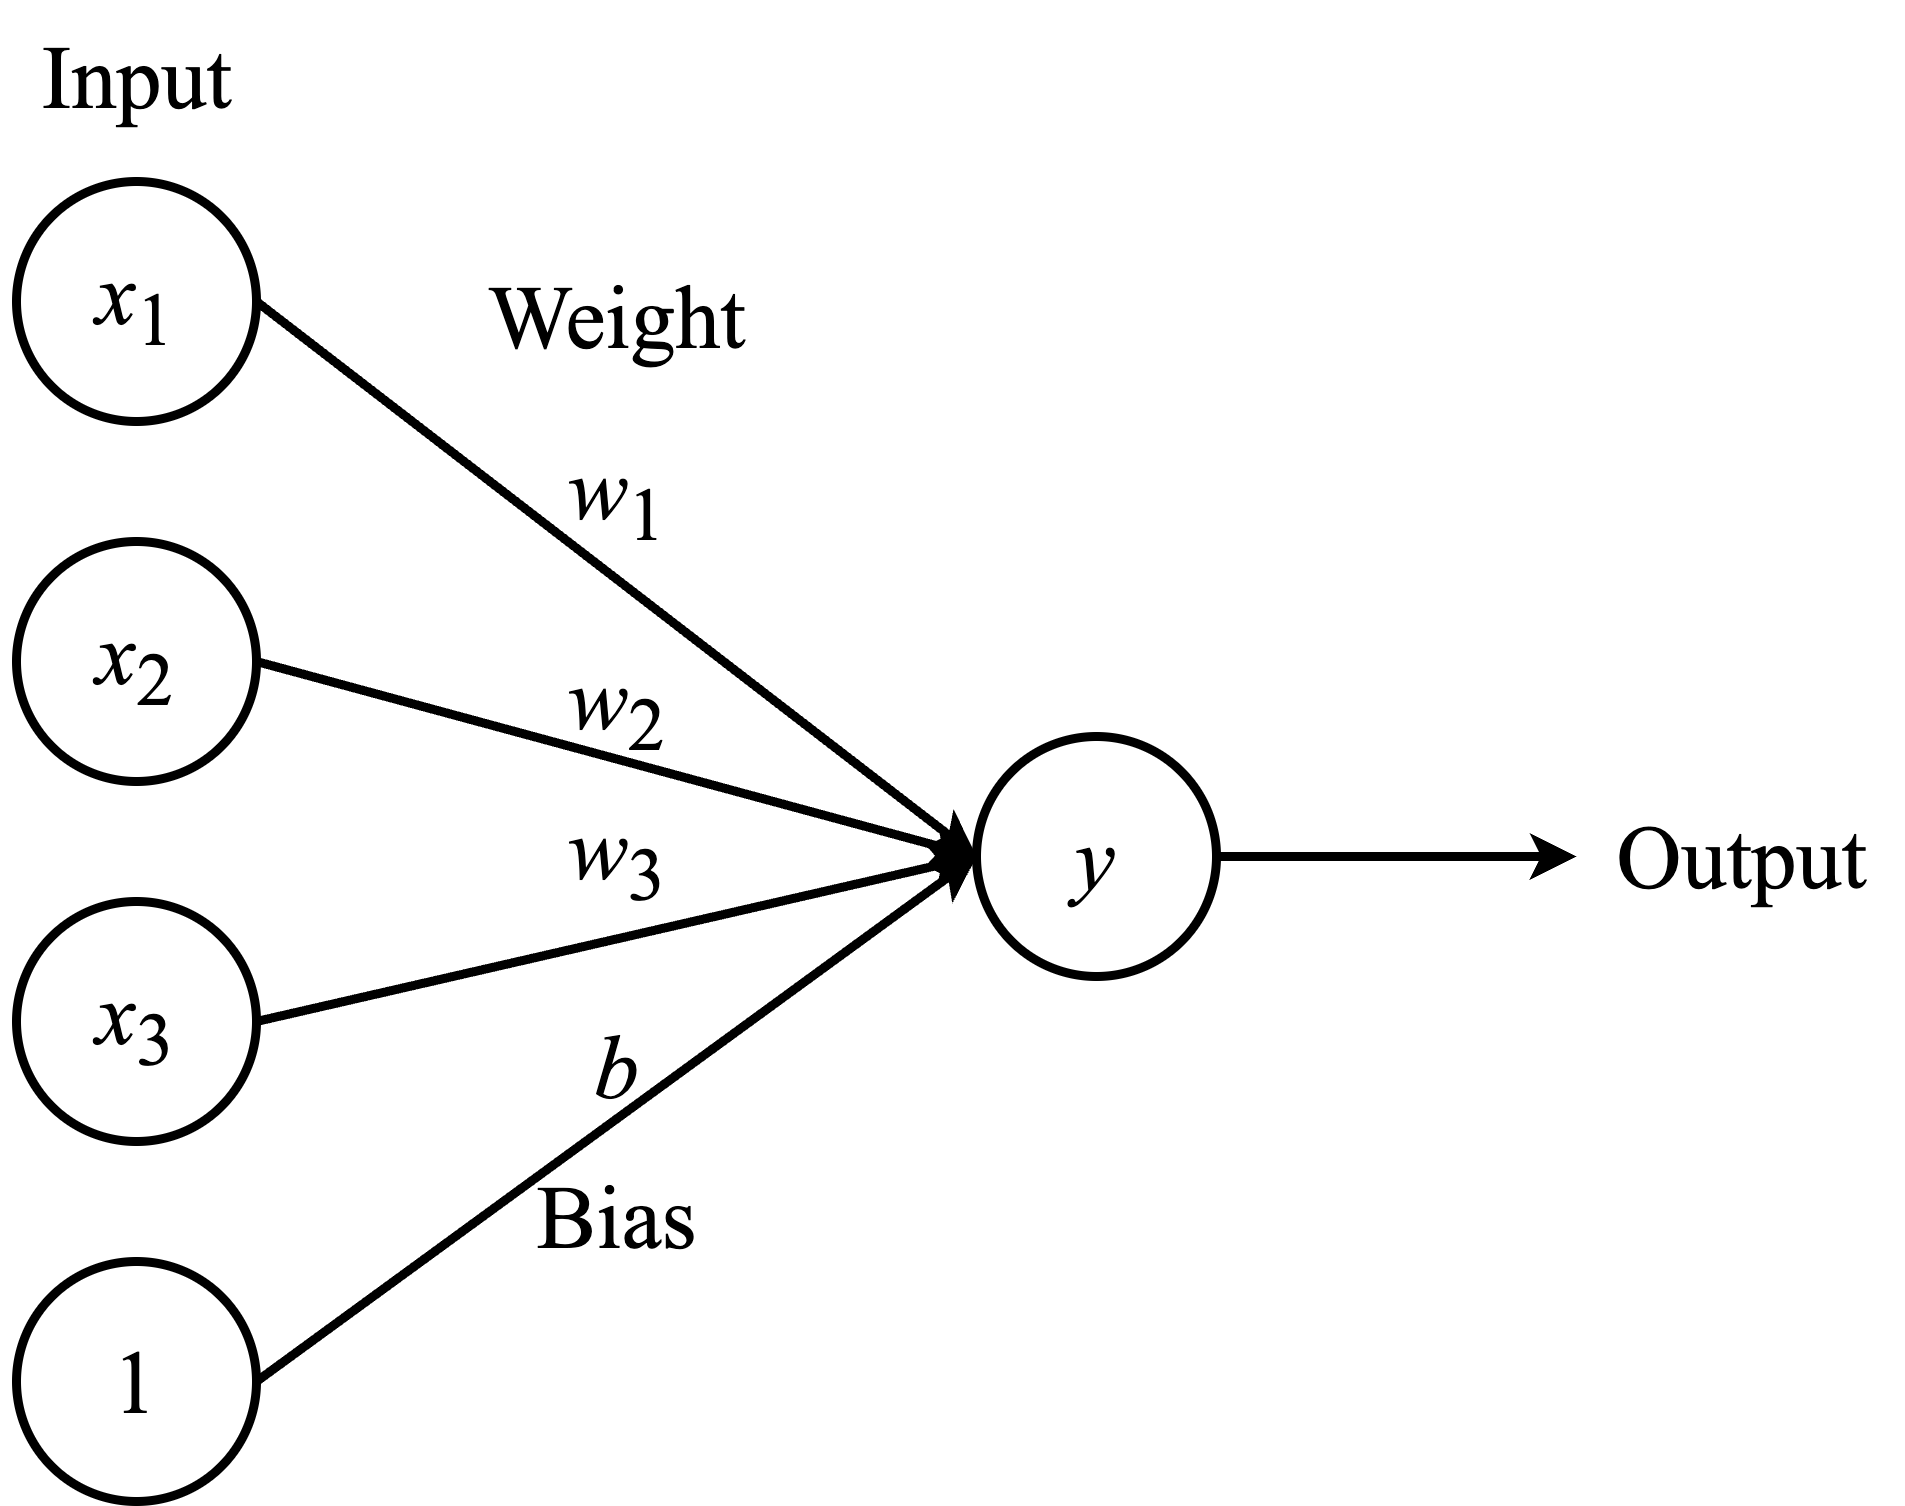
\includegraphics[scale = 0.13]{./chapter2/nn_1.png}
    \caption{ユニットの構造}
    \label{fig_NN1}
  \end{center}
\end{figure}

ここで出力$y$を複数個にすると,図\ref{fig_NN}のような構造になる.ユニットの縦方向の集まりのことを層と呼び,Neural Networkはこの層を複数組み合わせ,入力層・隠れ層・出力層という層を形成し計算を行う.
入力層$x$のユニットの個数を$i=1,2,3\ldots I$,隠れ層$z$のユニットの個数を$j=1,2,3\ldots J$とすると,それぞれの重みは$w_{j,i}$,バイアスは$b_j$となるため一般化した計算式は以下のようになる.
\begin{figure}[htbp]
  \begin{center}
    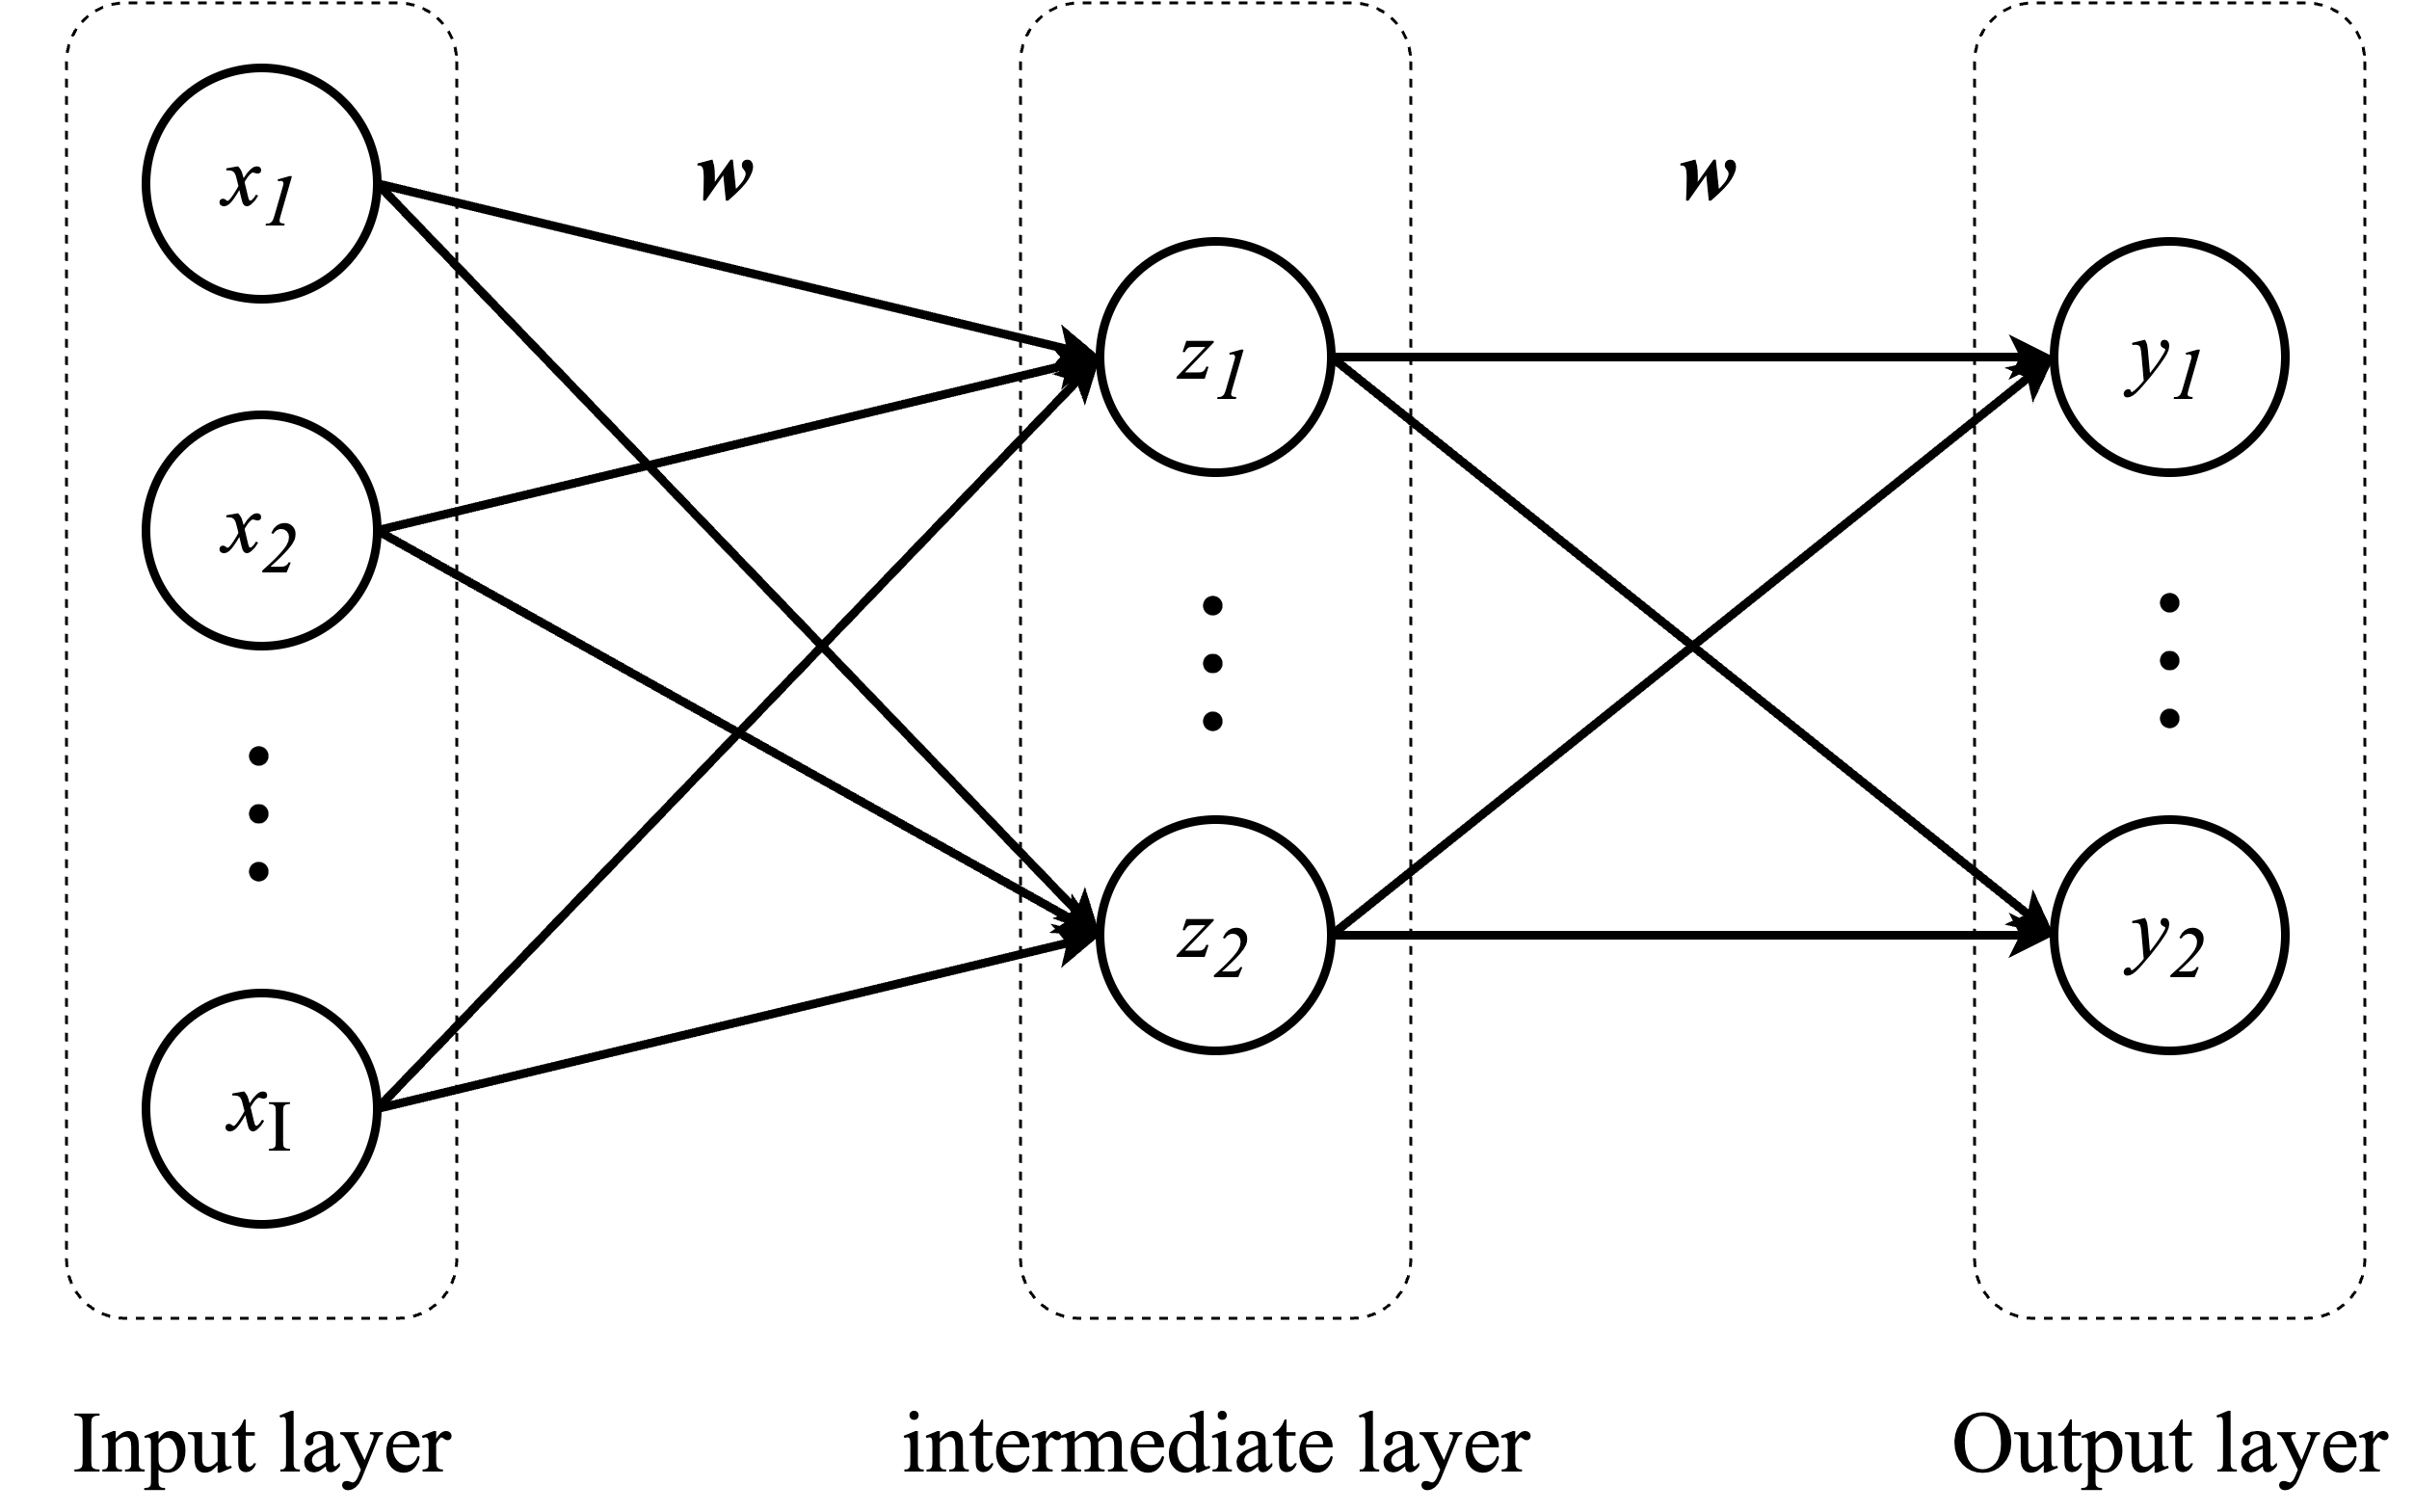
\includegraphics[scale = 0.13]{./chapter2/neural_network.png}
    \caption{Neural Networkの構造}
    \label{fig_NN}
  \end{center}
\end{figure}

\begin{align}
z_{j} &= \sum^{I}_{i=1}w_{j,i}x_{i} + b_j
\end{align}

ここで,各要素をベクトルと行列を用いて表し,次の層のユニットへの出力を一般化すると以下のような式となる.
\begin{align}
\bm{z} = \bm{W}\bm{x} + \bm{b}
\end{align}

隠れ層は1層のみである必要はなく,隠れ層の出力を次の層への入力として扱うことで層を多数化し,入力層から出力層までに多数の隠れ層を追加する.層数$L$のネットワークが存在する時,$l+1$層のユニットの出力$\bm{z}^{(l+1)}$は$l$層のユニットの出力$\bm{z}^{(l)}$から計算されるため,
\begin{align}
\bm{z}^{(l+1)} = \bm{W}^{(l+1)}\bm{z}^{(l)} + \bm{b}^{(l+1)}
\end{align}
という式で一般化される.したがって$l=1,2,3\ldots L-1$までの計算を順に行なっていくことで各層の出力を得ることができ,最終的な出力$\bm{y}=\bm{z}^{(L)}$を計算することができる.このような構造の層を全結合層と呼ぶことが多い.


\subsection{学習による重みの更新}
前項のような計算により,入力が与えられたときの出力を得ることができ,このときの出力がNeural Networkが導いた推論になる.教師あり学習の場合,入力に対し求められる出力が正解として与えられる.その正解と,入力からネットワークによって求められた推論を比較し,より求められる正解に推論が近づくように重みを更新していくのである.

例えば0から9までの手書き文字が入力として与えられその分類を行うとき,出力は$y_0, y_1, \ldots , y_9$までの10個の出力を用意する.10個の出力に対し0から9までの数字を対応させ出力が1になった数字を推論として扱う.その時の構造を図\ref{fig_study}に示す.
\begin{figure}[htbp]
  \begin{center}
    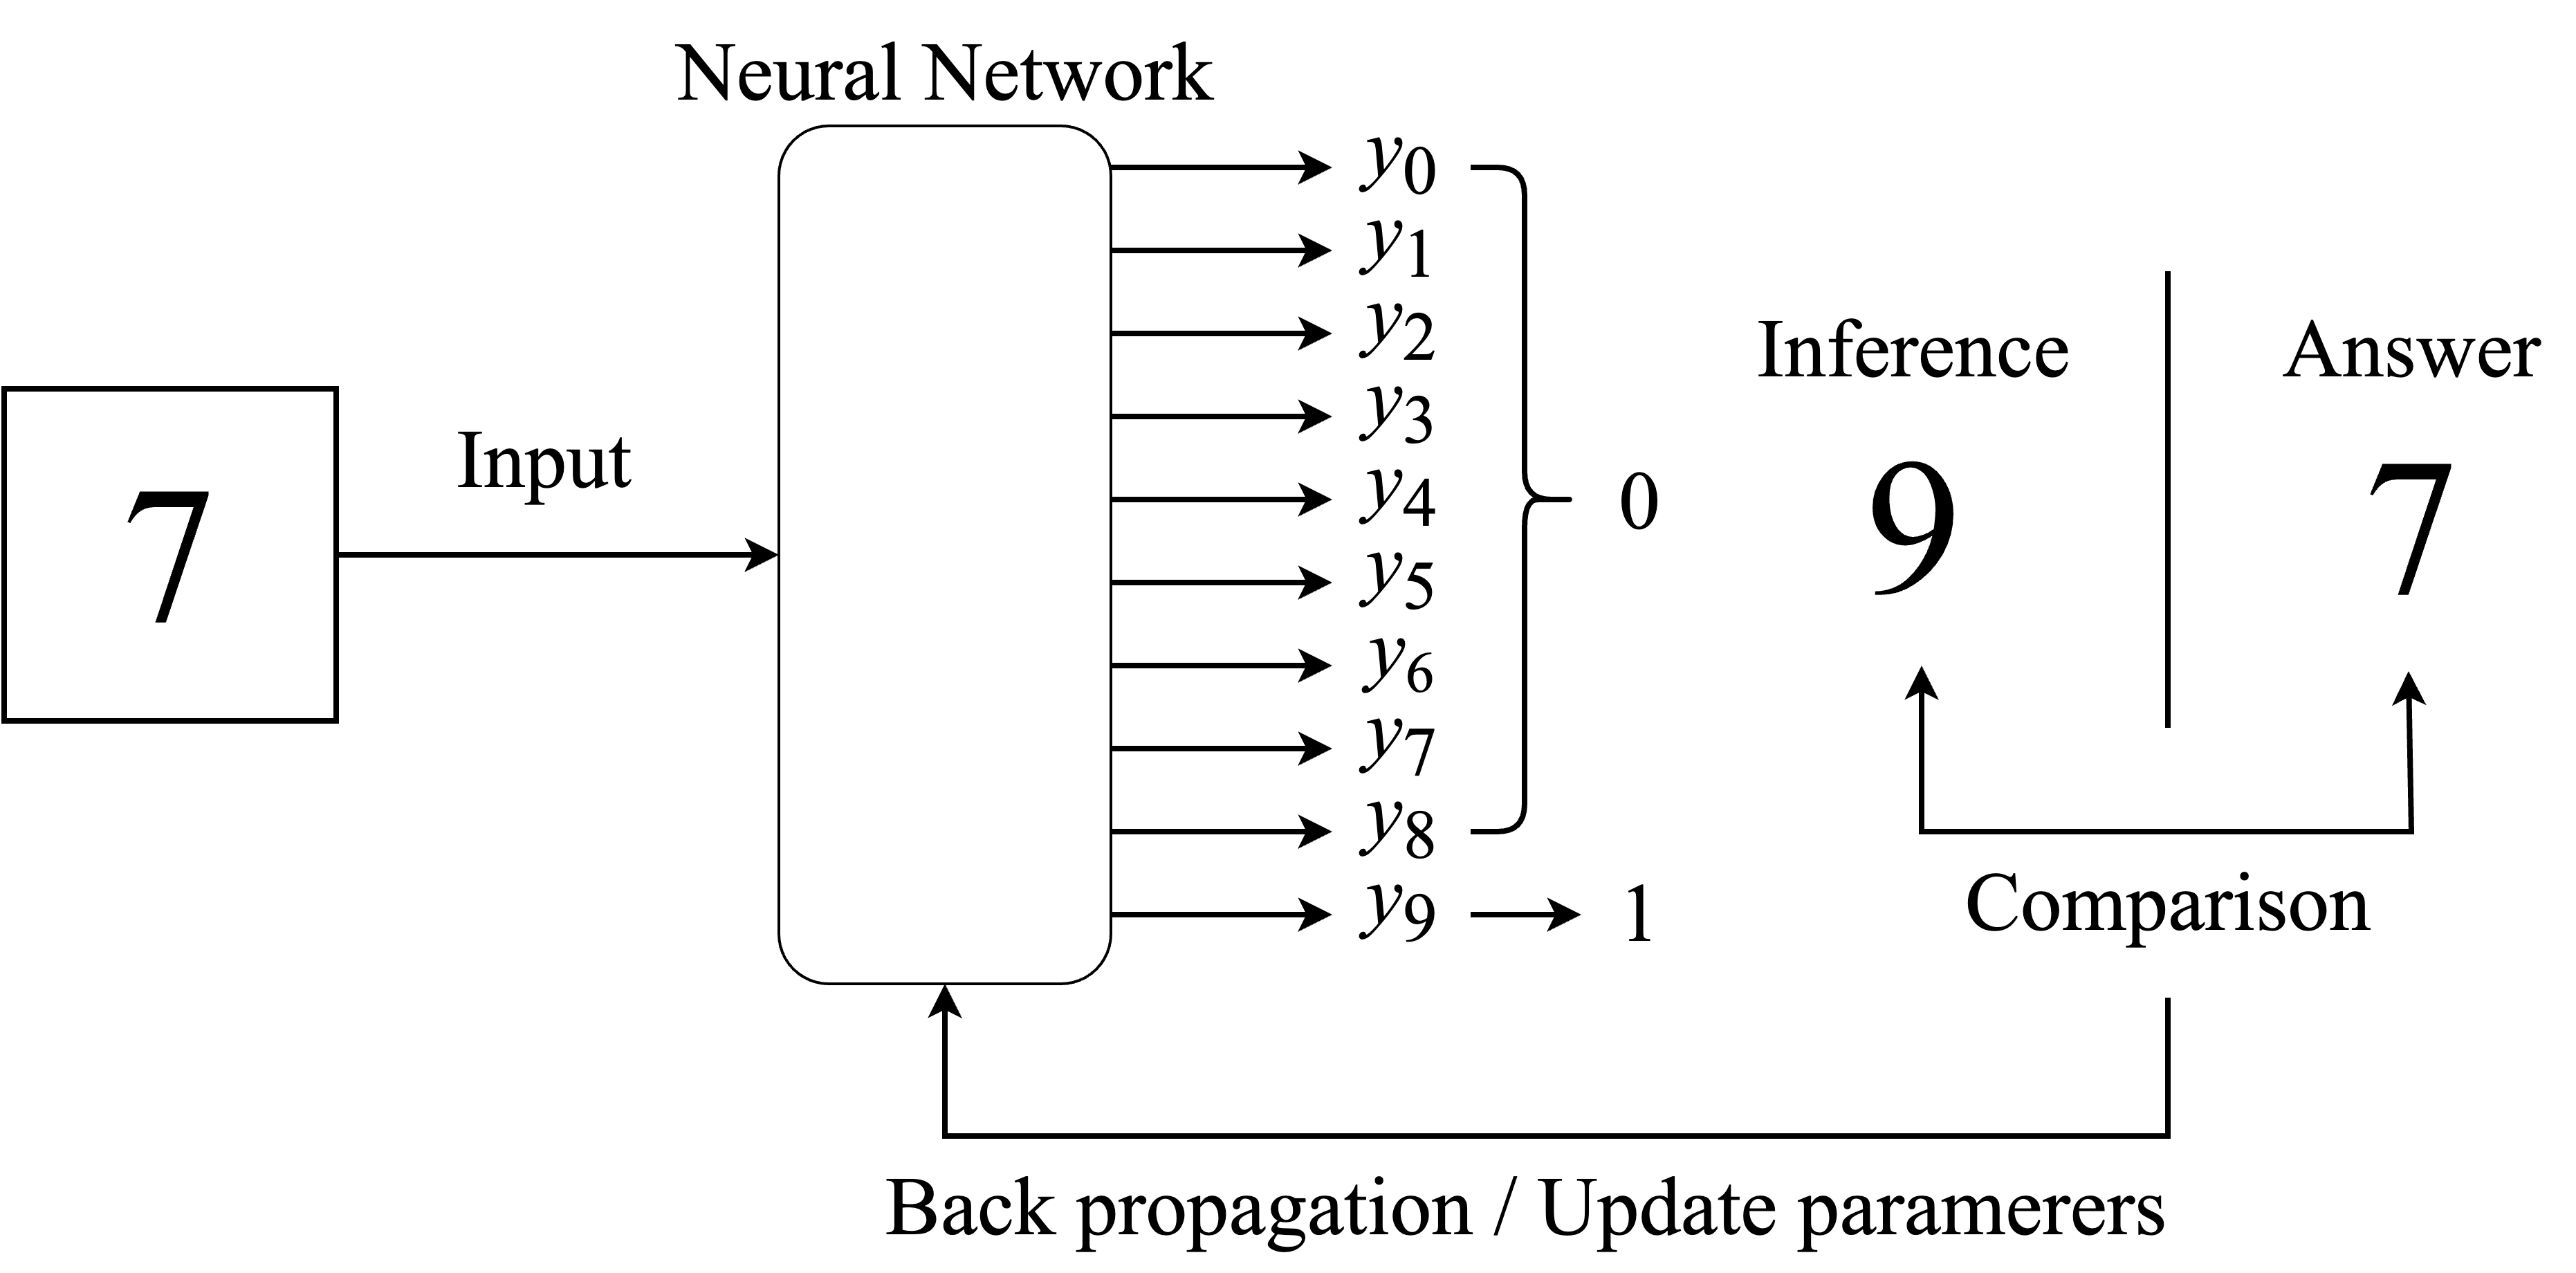
\includegraphics[scale = 0.1]{./chapter2/NN_study.png}
    \caption{Neural Networkにおける学習の流れ}
    \label{fig_study}
  \end{center}
\end{figure}

このとき,実際の答えは7だが推論の結果は9となり不正解になる.そこで両者を比較し誤差逆伝搬を行うことでNeural Network内の重みをどのように変更すれば推論を正解に近づけることができるかを求める.そして重みを更新していき推論が正解に近づいていくように変更していくのがNeural Networkにおける機械学習である\cite{sinsou}.

% ******************************************************
% CNN
% ******************************************************
\section{CNN}
\subsection{学習の概要}
CNNとは畳み込みと呼ばれる画像処理を組み込んだNeural Networkの1種で,画像分類など画像を用いた学習を得意としている.Neural Networkに畳み込み層を追加したものがCNNであるが,畳み込み層における画像,フィルタがNeural Networkにおける入力,重みとなっている.
CNNでは主に畳み込みとプーリングという処理を用いて画像の特徴を抽出し学習を行っている.


\subsection{畳み込み}
畳み込みとは画像に対してフィルタをかけ,フィルタと類似する濃淡パターンを検出する役割を持つ.
畳み込み層を考える上で,図\ref{fig_conv}のように$I \times J$ピクセルの画像と$2 \times 2$の要素を持つフィルタが存在すると考える.
\begin{figure}[htbp]
  \begin{center}
    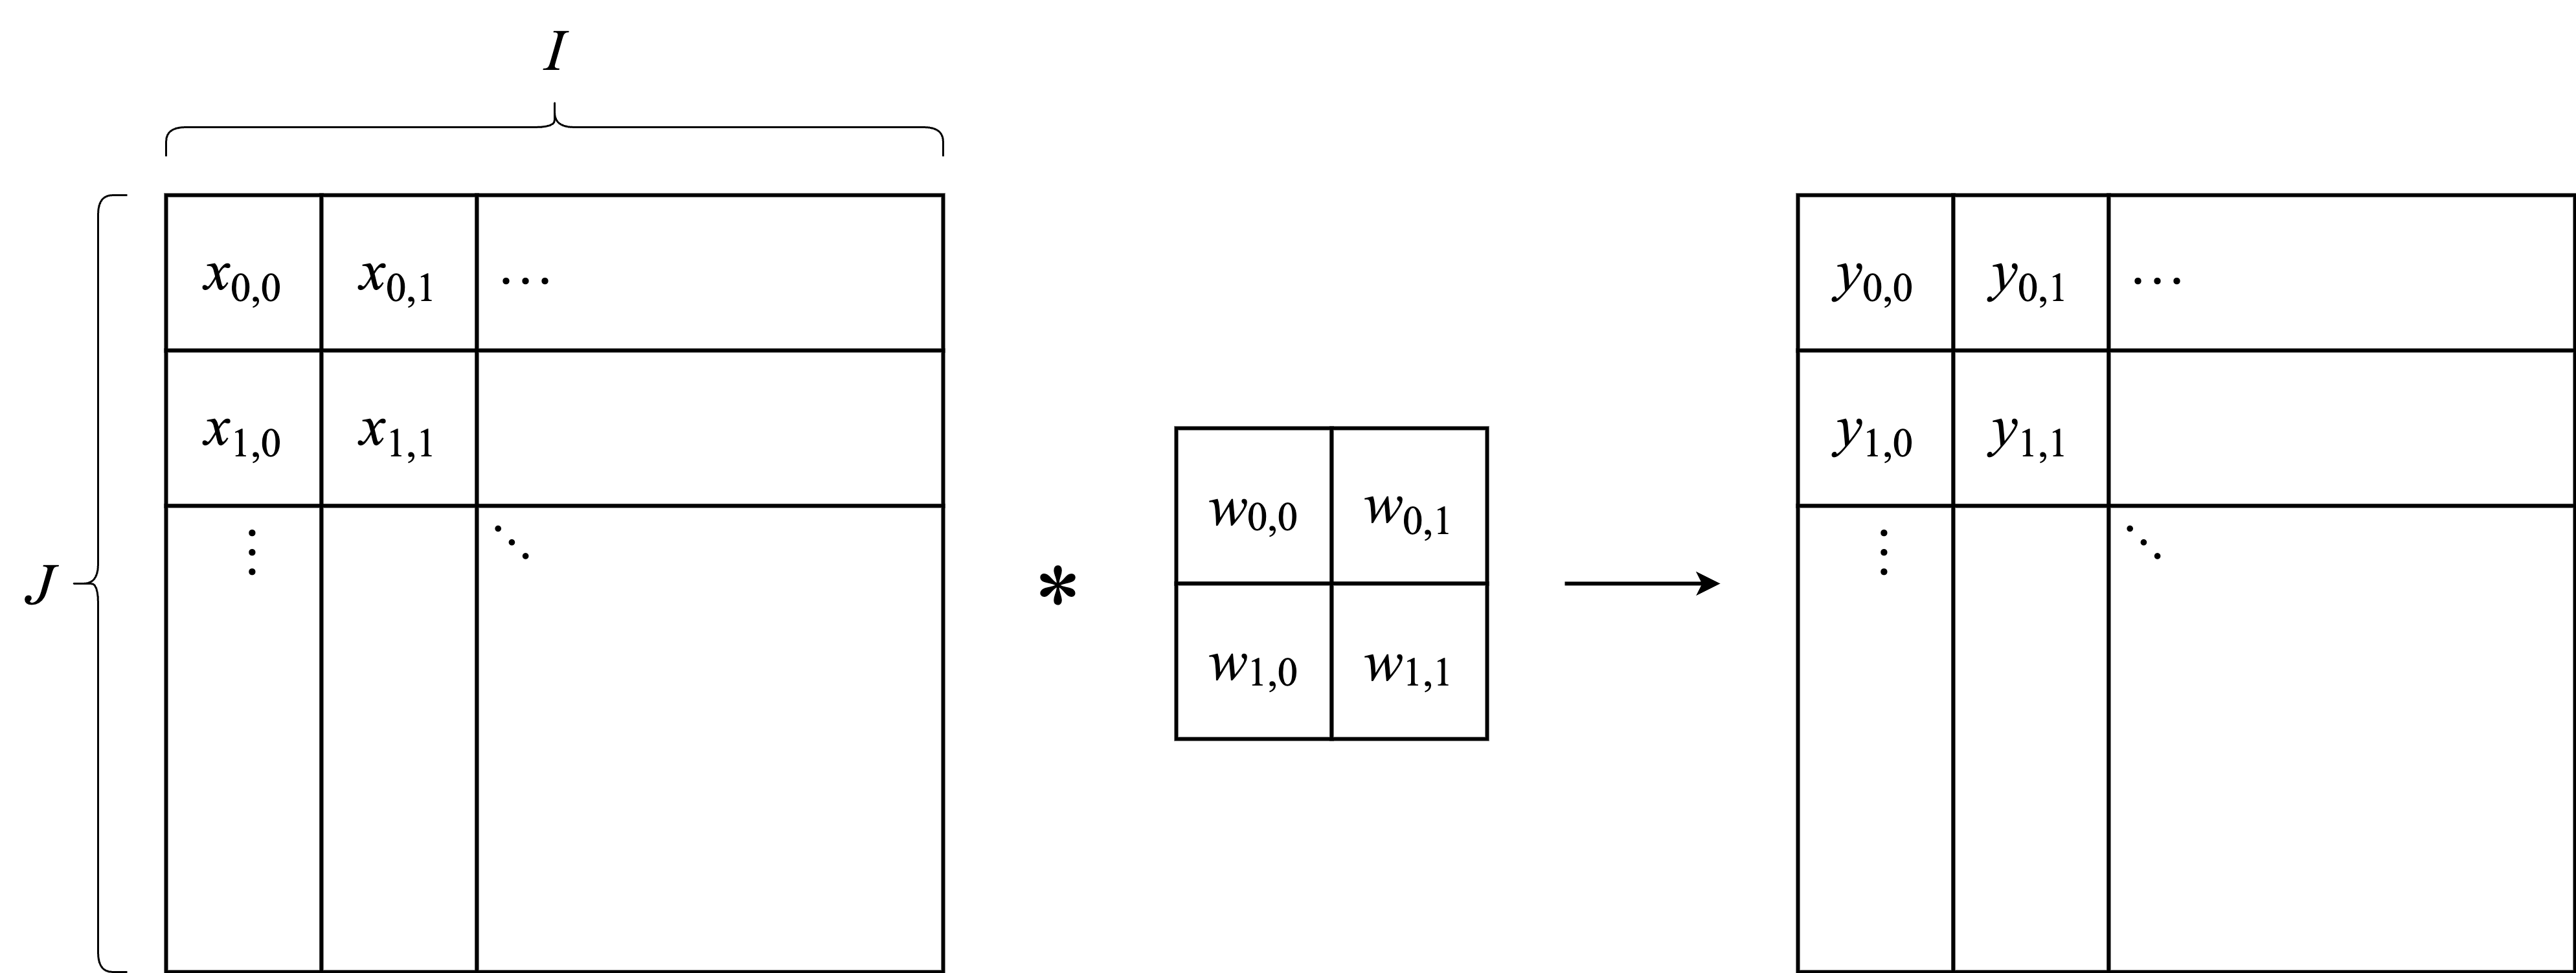
\includegraphics[scale = 0.1]{./chapter2/cnn_tatamikomi.png}
    \caption{畳み込みの計算}
    \label{fig_conv}
  \end{center}
\end{figure}

ここでフィルタを$x_{00}$に重ねるように置き,各要素について乗算したものの和を出力とすると以下のように計算できる.
\begin{align}
  y_{0,0} = x_{0,0}w_{0,0} + x_{0,1}w_{0,1} + x_{1,0}w_{1,0} + x_{1,1}w_{1,1}
  \label{fig_NN1}
\end{align}

畳み込み層ではフィルターを1ピクセルずつスライドさせながら同じ計算をする.出力$y$のインデックスを$i,j$とし,フィルタのサイズを$W\times H$,とすると出力は以下の式で一般化できる.
\begin{align}
  y_{i,j} = \sum^{W-1}_{p=0} \sum^{H-1}_{q=0} x_{i-p,j-q}w_{p,q}
\end{align}
CNNではこの計算を繰り返していくことで画像の特徴を抽出する.

このままでは入力の画像に対し出力画像が1ピクセル分小さくなってしまうため,前後で画像サイズを変更したくない場合はパディングと呼ばれる入力画像の外側に情報を追加する処理を行う.よく使用されているのは0パディングと呼ばれる画像の外側1ピクセル分を0で埋め尽くす処理である.

また,通常のNeural Networkと同様に入力には複数枚の画像を使用する.複数の画像に同一のフィルタを畳み込み,それを足し合わせることで出力を得る.フィルタは層ごとに増やしていき,フィルターの数だけ画像のch数は増えていく.これを図に表すと図\ref{fig_cnn_ch}のようになる.
\begin{figure}[htbp]
  \begin{center}
    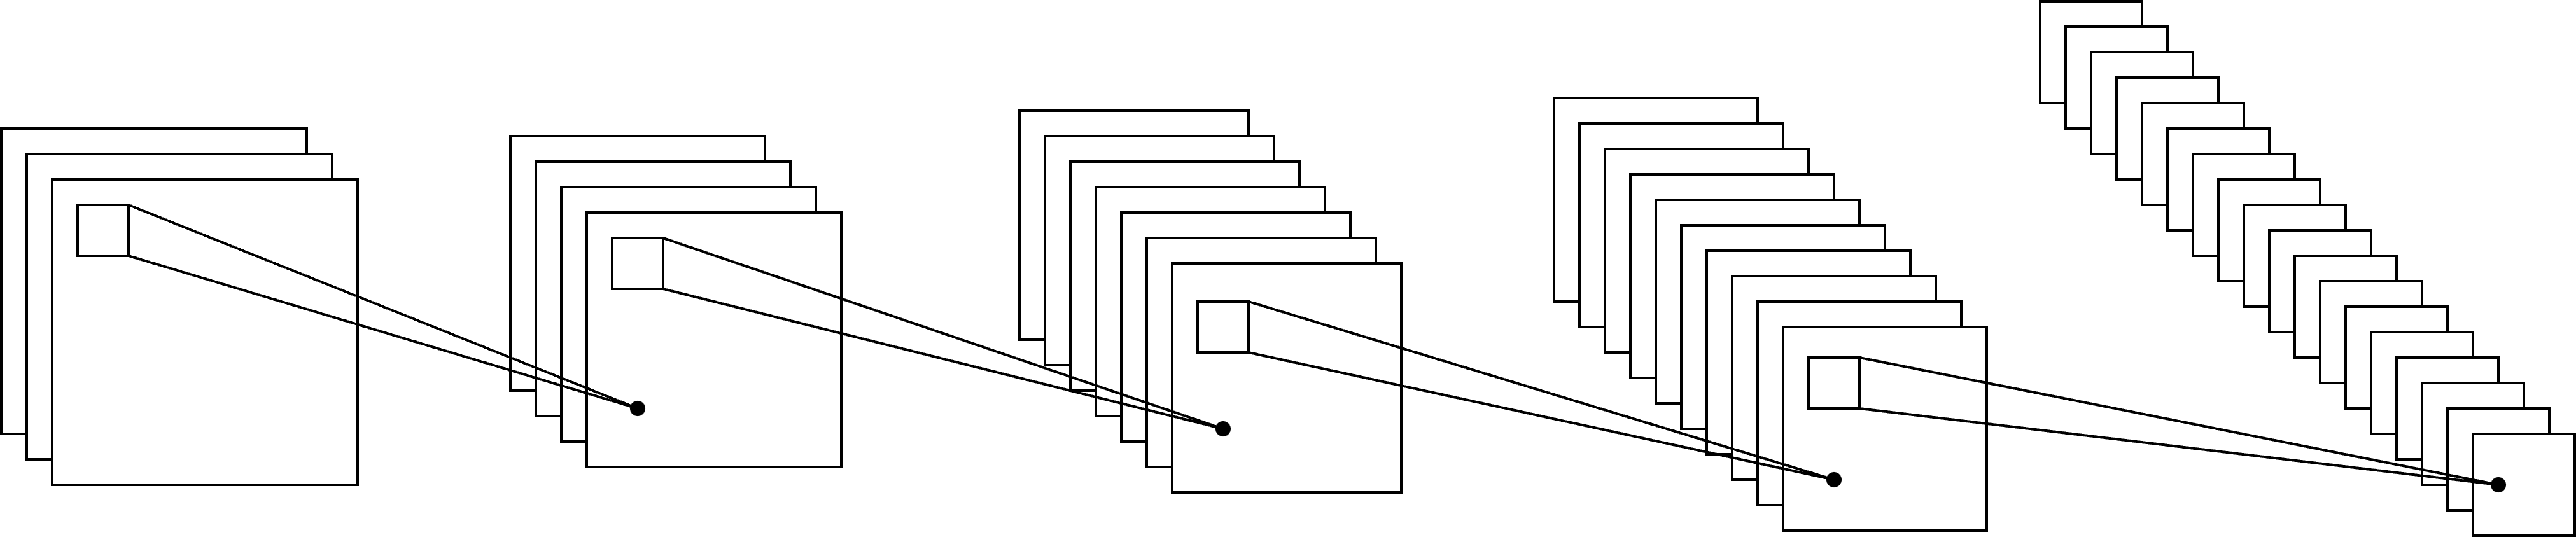
\includegraphics[scale = 0.05]{./chapter2/cnn_ch.png}
    \caption{畳み込み層での計算の概要}
    \label{fig_cnn_ch}
  \end{center}
\end{figure}

\subsection{プーリング}
プーリングとは畳み込みで取得した画像の特徴を増幅させるような処理である.畳み込みを行った画像に対し,あらかじめ指定したサイズで画像を分割しその分割ごとに情報を要約することと,解像度を落としダウンサンプリングさせるような2つの効果を持つ.この2つの処理によって入力信号の平滑化とダウンサンプリングによるエイリアシングの防止をになっている.

プーリングにはいくつかの種類が存在する.その中でも最も一般的な手法が図\ref{fig_pooling}に示すような最大値プーリングである.これは入力画像を指定したパディングサイズごとに分割して,その分割内の最大値を出力とする手法である\cite{sinsou}.
\begin{figure}[htbp]
  \begin{center}
    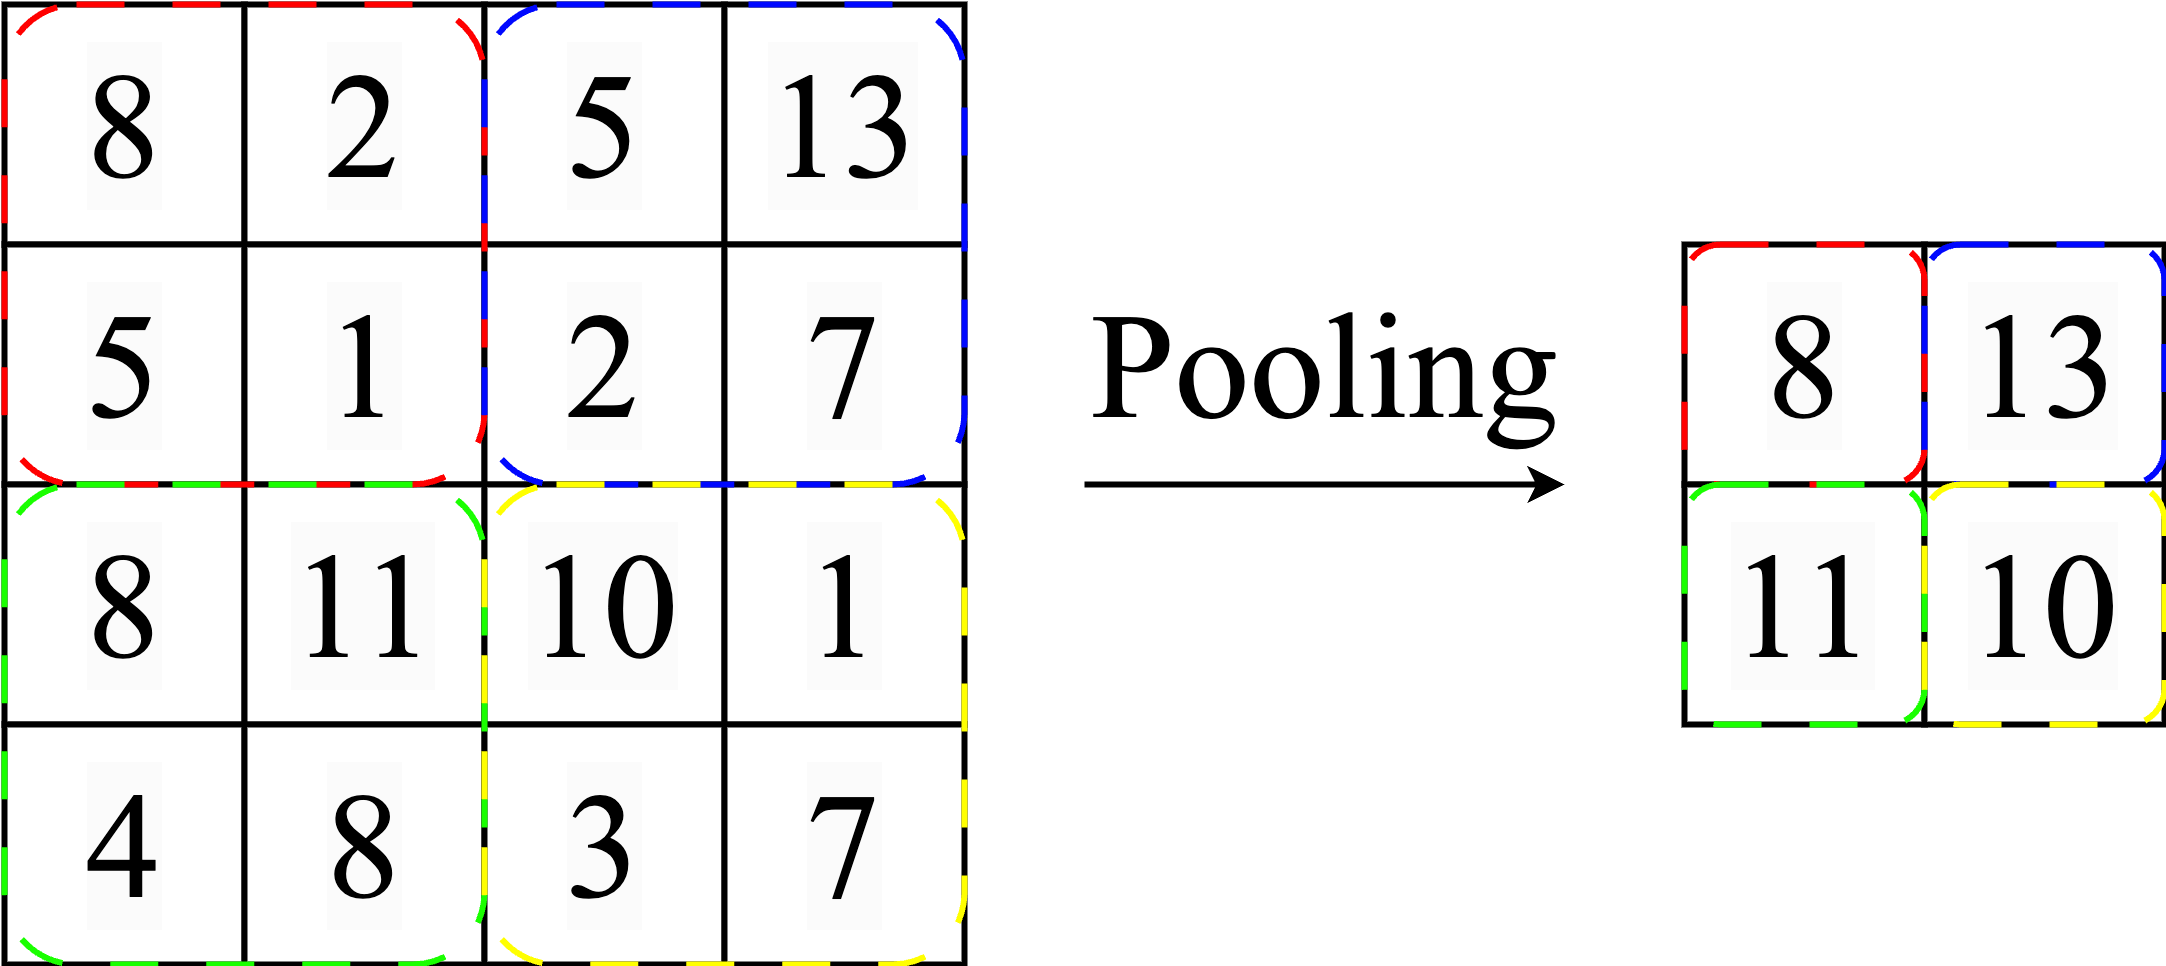
\includegraphics[scale = 0.13]{./chapter2/pooling.png}
    \caption{最大値プーリング}
    \label{fig_pooling}
  \end{center}
\end{figure}


% ******************************************************
% BinaryConnect
% ******************************************************
\section{BinaryConnect}
BinaryConnectとはNeuralNetworkにおける重みを1と-1に2値化する手法である.浮動小数の重みを$\bm{w}$,2値化した重みを$\bm{w}_b$とすると,$\bm{w}_b$は以下のように計算される.
\begin{displaymath}
  \bm{w_{b}} = \left\{ \begin{array}{l}
  \displaystyle 
  +1\:  \text{if}\:  \bm{w} > 0 \\
  -1\:\text{otherwise}
  \end{array} \right.
\end{displaymath}

通常のNeural Networkの重みは32bitまたは16bitの浮動小数点で表されるが,BinaryConnectでは1,-1ネットワーク内で0,1に対応させ,1bitで表すことができる.これにより重みのメモリ使用量は32分の1まで抑えることが可能である.

また,前章より図\ref{fig_conv}での畳み込み層での計算は式\ref{fig_NN1}で計算されるが,重みを全て1,-1にすることによって以下の式のように入力と重みの乗算を加減算のみで表すことができるようになる.
\begin{align}
  y_{0,0} = x_{0,0} \pm x_{0,1} \pm x_{1,0} \pm x_{1,1}
\end{align}
これにより,ネットワーク中の乗算器を加算機に置き換えることができるため計算リソースの削減をすることができる

学習における勾配の蓄積や重みの更新は一般的なCNN通り,浮動小数の重みに対して処理し,推論時に使用する重みのみ2値化の処理をする.図\ref{fig_binarize} に処理の流れを示す\cite{courbariaux2016binaryconnect}.
\begin{figure}[htbp]
  \begin{center}
    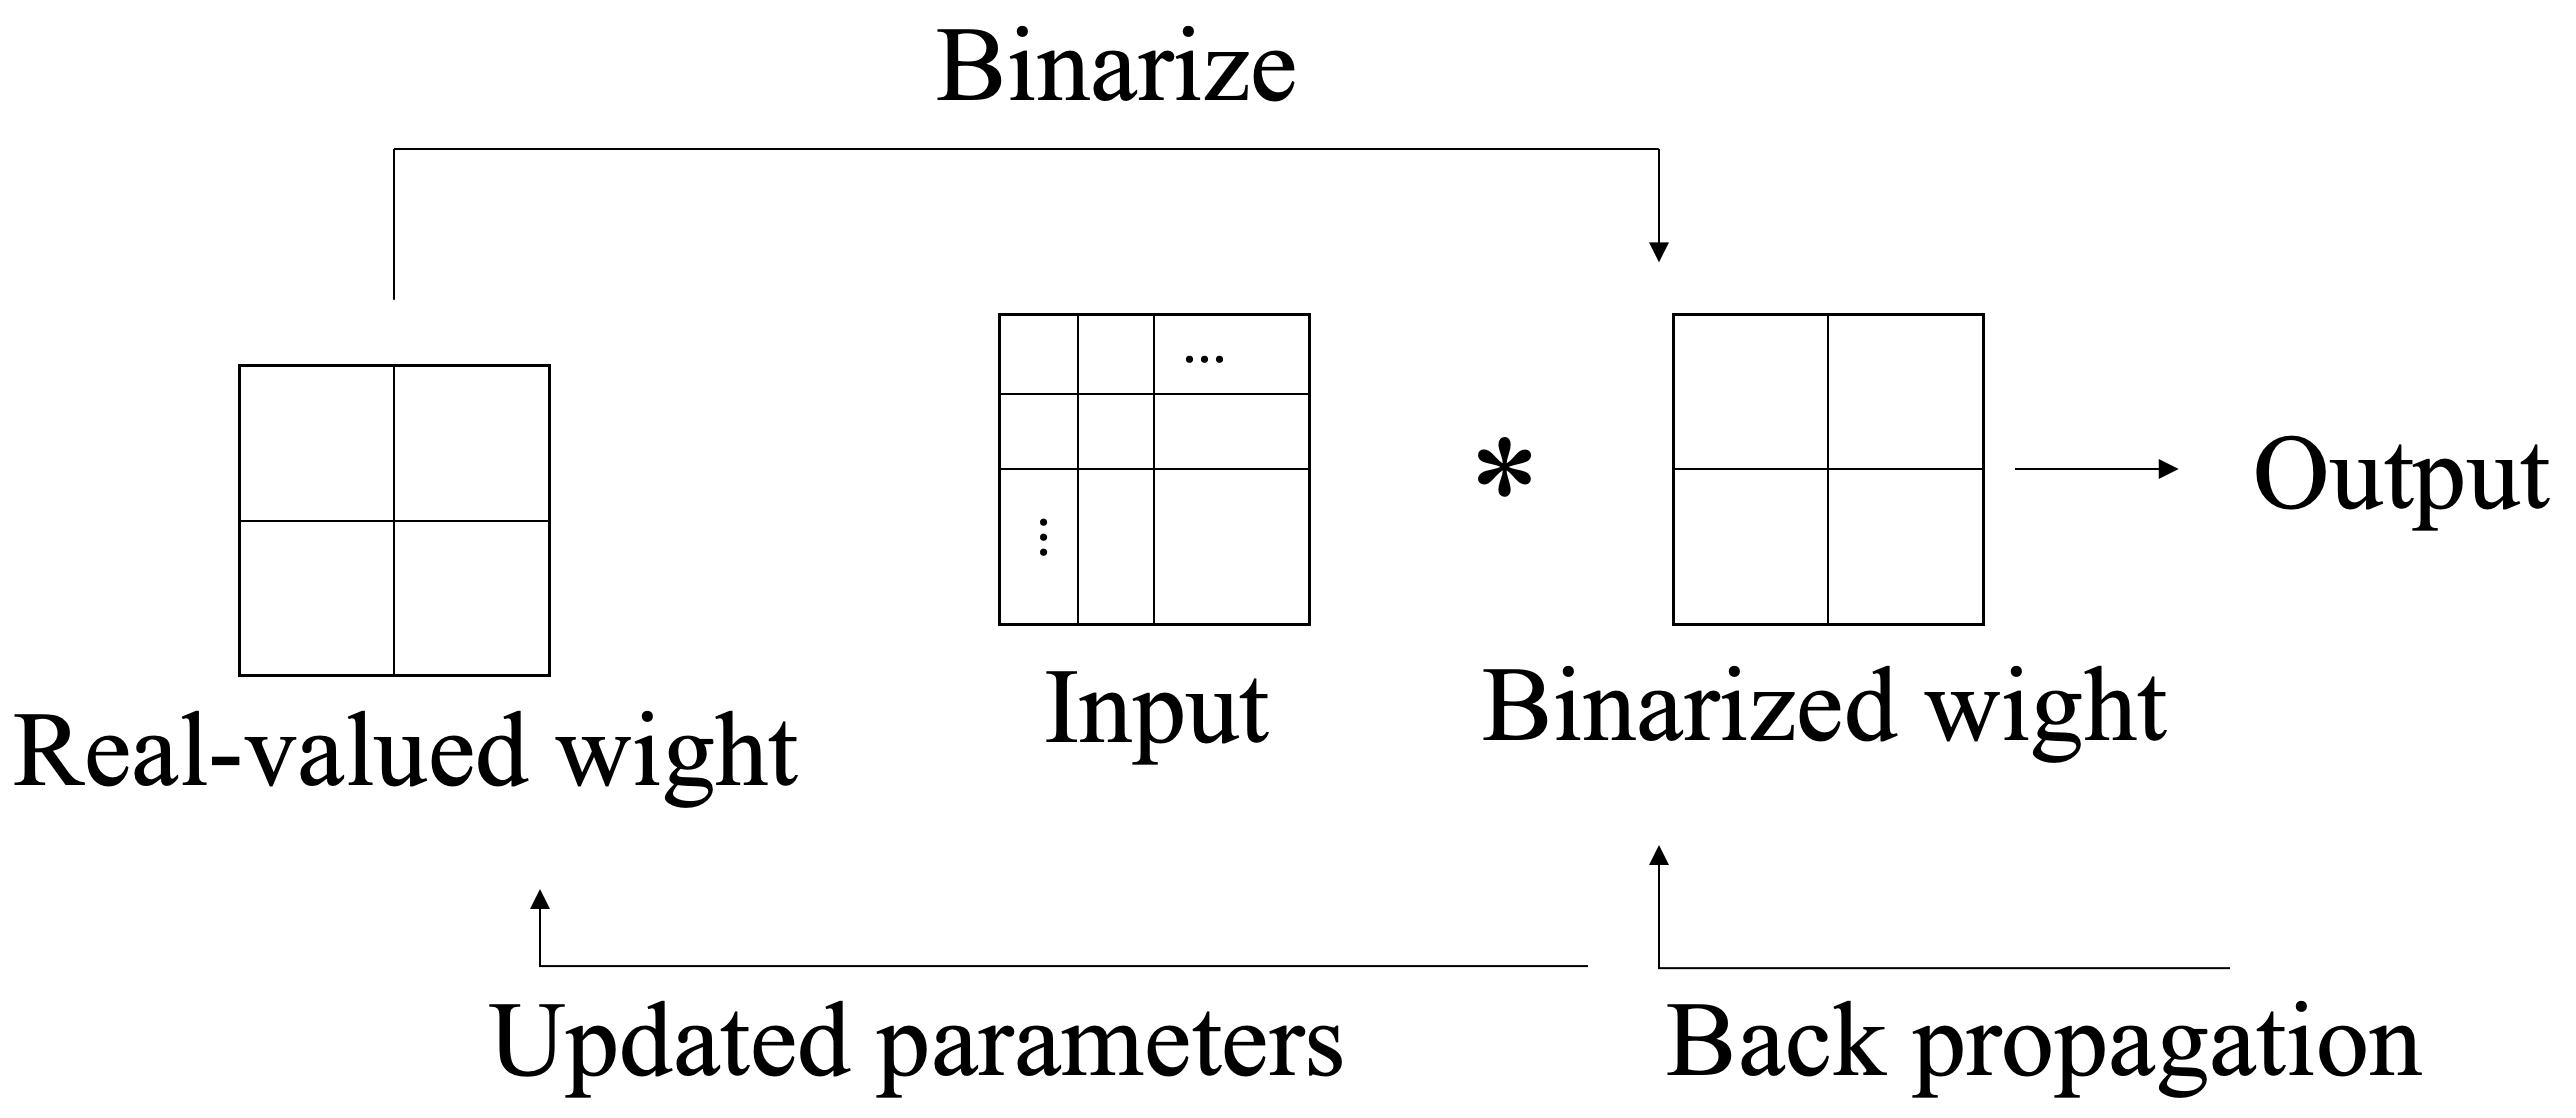
\includegraphics[scale = 0.25]{./chapter2/binarize.png}
    \caption{BinaryConnectにおけるパラメータ更新の流れ}
    \label{fig_binarize}
  \end{center}
\end{figure}

% bibtex 
% {}内を{junsrt}にしないと引用順番にならないので注意
\bibliographystyle{junsrt}
% 関連図書 → 参考文献に変更する
% jbook.clsのthebibliographyは、関連図書と出力するので、
% 		\renewcommand{\bibname}{参考文献}
%  をプレアンブルに入れることで、"参考文献"と変わります。jarticleの場合は、
 % 		\renewcommand{\refname}{参考}

\renewcommand{\bibname}{参考文献}
\bibliography{./etc/ref}
% 以下のように複数ある場合は複数指定できる
% \bibliography{./etc/ref,./etc/ref_2}

% 謝辞

\chapter*{謝辞}
本研究の実施にあたり,ご指導くださった米子工業高等専門学校電子制御工学科内田雅人講師に感謝申し上げます.

% ================================================
% Document (end)
% ================================================

\end{document}

